\subsubsection{20.02.2016}
\textit{\textbf{Time frame:}} 10:00-21:00 

It was the second day of the competition. Today were held only qualification matches. Our team participated in 4 matches and we managed to win in all of them.

\begin{figure}[H]
	\begin{minipage}[h]{0.47\linewidth}
		\center{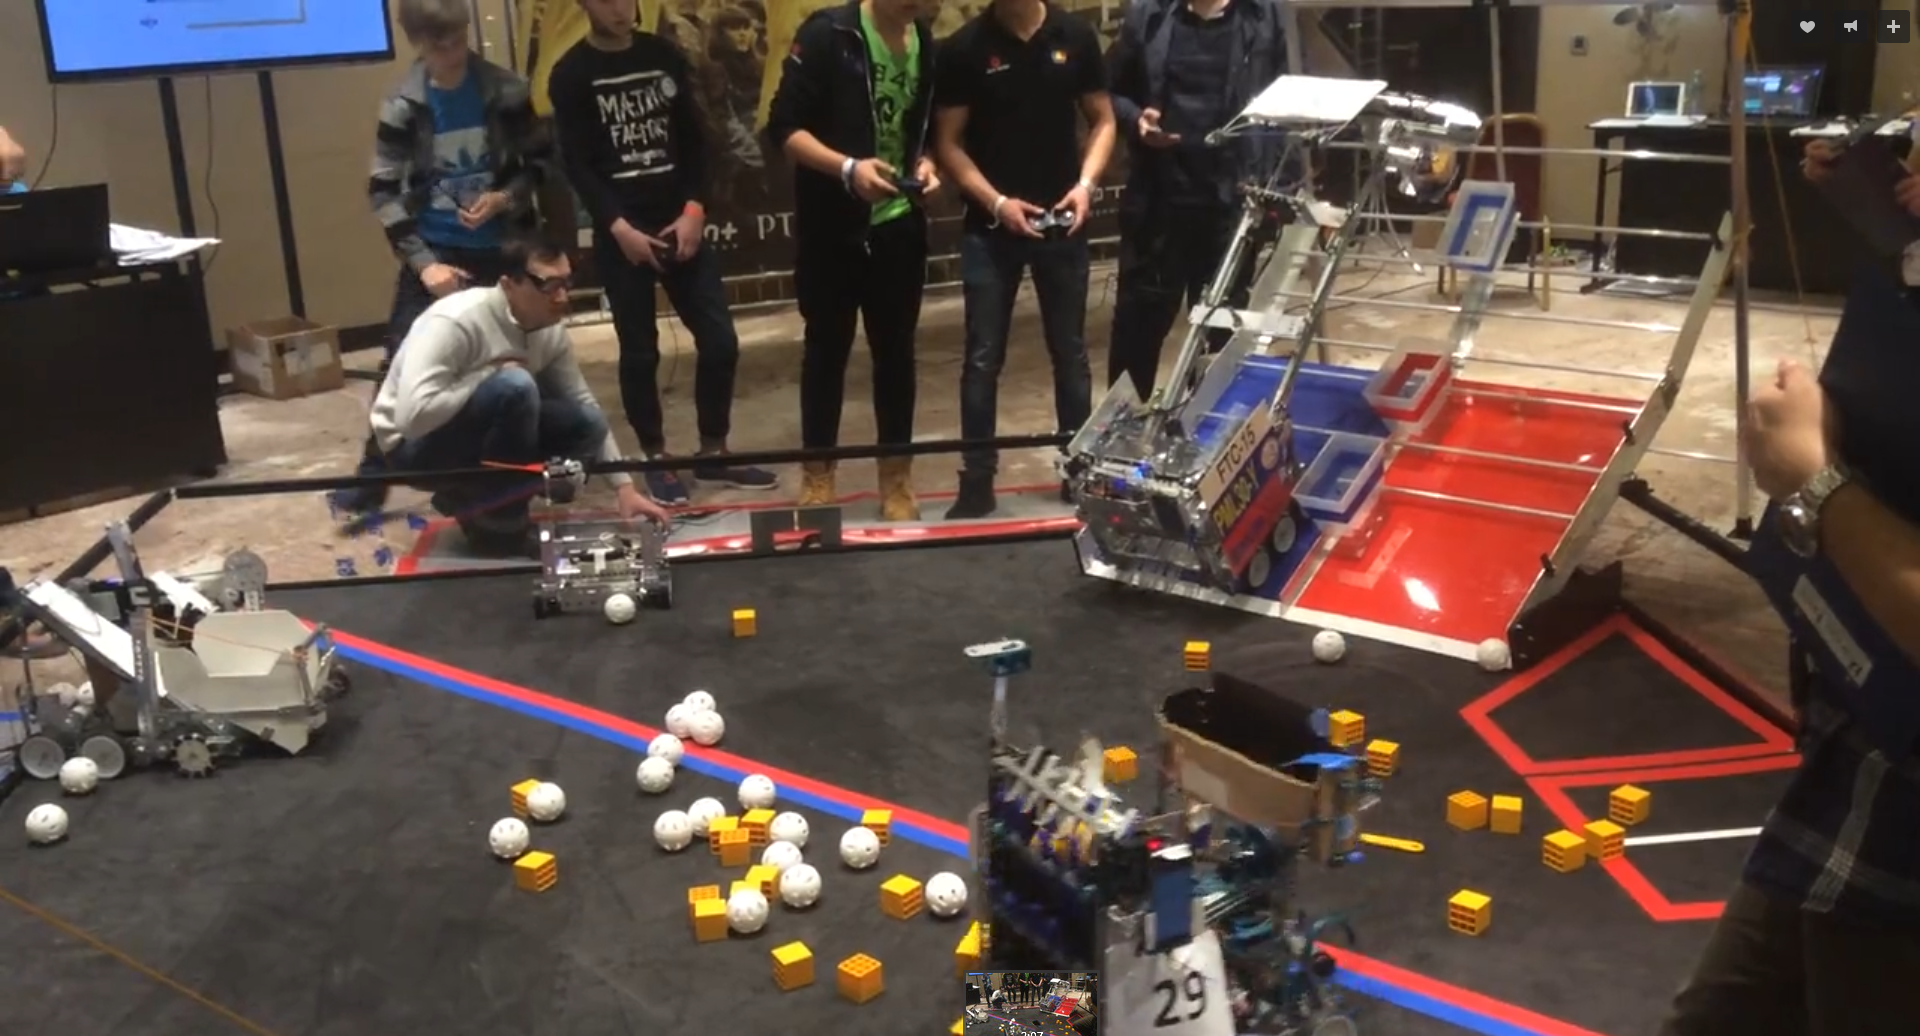
\includegraphics[scale=0.17]{3Engineering/5Team_meetings/days_of_meetings/2016.02.20/images/01}}
		\caption{Match in progress. Our robot is scoring debris into the top goal}
	\end{minipage}
	\hfill
	\begin{minipage}[h]{0.47\linewidth}
		\center{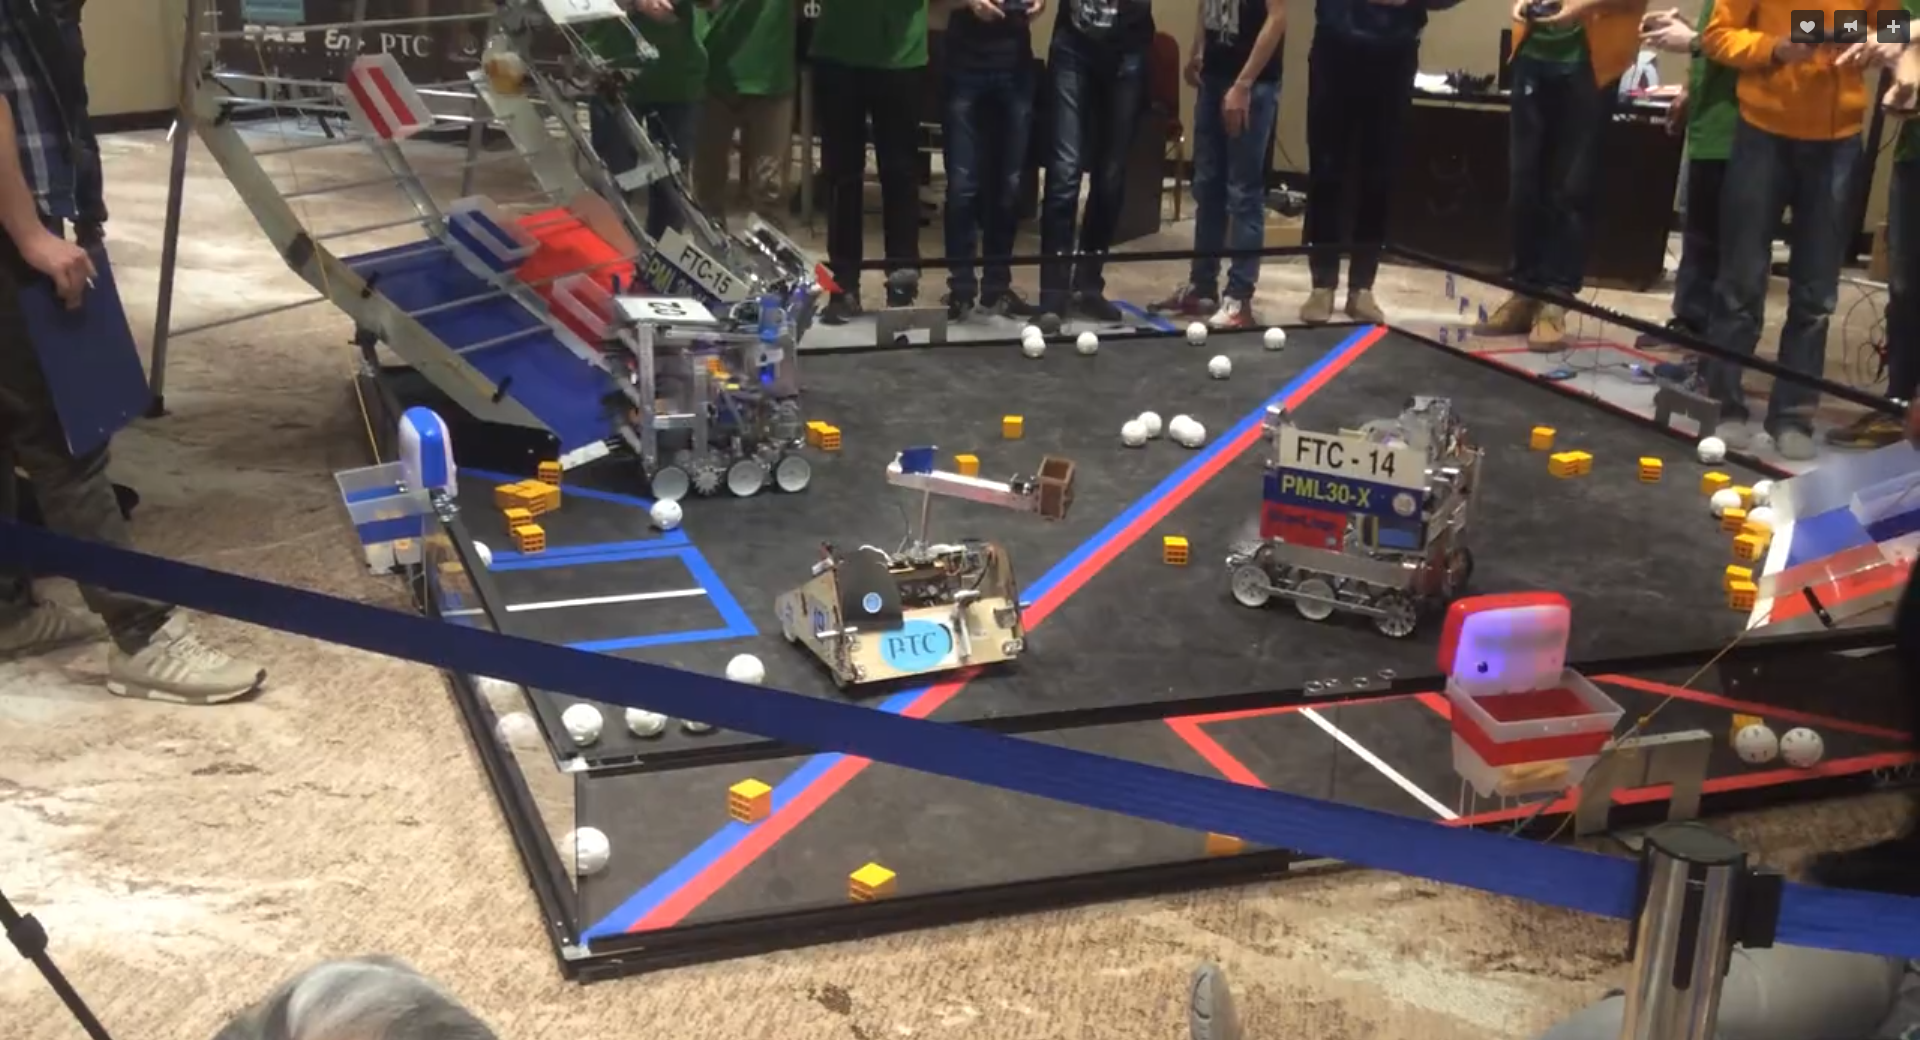
\includegraphics[scale=0.17]{3Engineering/5Team_meetings/days_of_meetings/2016.02.20/images/02}}
		\caption{Another match}
	\end{minipage}
\end{figure}

During the matches it was found out that the "All Clear" signal fixed tighter that we expected and it required strong force to turn it. Our mechanism for pushing the baton was not strong enough to turn the baton on the official field. Due to this fact, it was decided to remove the mechanism for pushing the "All Clear" signal from the robot.